% !TEX root = ../foresight.tex

\section{Relative pose localization}

From each UWB tag we receive a range measurement $r_i$ in its own frame. 
From the quadrotor we receive velocity measurements $\bm{v}$, a yaw reading $\psi_q$,
and an altitude measurement $z_a$ in an ENU-aligned world frame. The frames and relative
transforms of our system are visualized in Fig.~\ref{fig:frames}.
Given $n$ UWBs, we define the measurement vector as $z = [r_1, \dots, r_n, \bm{v}, z_a, \psi_q] \in \R^{n+5}$

%We use 6 ultra-wideband radios and the Bebop's onboard odometry measurements
%to estimate the relative position of the quadcopter with respect to the car with an
%accuracy of 13 cm. The 6 UWBs were positioned as far apart as possible on the
%car while still maintaining line of sight with the quadcopter when the
%quadcopter is positioned in front of the car. The transform from a set base position
%on the car to each UWB was then measured. These transforms allow us to
%calculate the distance between each UWB and the estimated state of the quadcopter.


Yaw orientation is calibrated at the start by lining up the quadrotor along the car's x-axis
and measuring the yaw offset $\psi_{\text{off}}$ between the car and the quadrotor.
The yaw of the quadrotor is then given by $\psi = \psi_q - \psi_{\text{off}}$

One challenge we encountered in estimating the 3D position of the quadrotor was that
the distance measurements from the UWBs showed larger errors when the UWB on the quadrotor was out of their plane.
We therefore first estimate $\bm{\hat{p}^{\text{odom}}}$ using only use the quadrotor's onboard 
odometry readings $\bm{v}$ and $z_a$ as the inputs to a UKF. We then use the estimated
height, $\bm{\hat{p}_z^{\text{odom}}}$ with the UWB range
measurements $r_i$ to estimate the quadrotor's x-y position, $\bm{\hat{p}^{xy}}$.
We do this by first projecting each $r_i$ onto the plane of the estimated height of the quadrotor:

$$
   r_i^{\text{proj}} = \sqrt{r_i^2 - (\bm{\hat{p}_z^{\text{odom}}})^2}
$$

We then find $\bm{\hat{p}^{xy}}$ by solving the nonlinear least squares optimization

\begin{align*} 
    h(\bm{\hat{p}^{xy}}) = \min_{{\bm{\hat{p}^{xy}}}} \sum_{i=1}^{n} ((r_{i}^{\text{proj}})^2 - \lVert \bm{\hat{p}^{xy}} - \bm{t_i^{xy}}\rVert^2)^2
\end{align*}

% with the Jacobian \ja{with respect to what? P? If so, I think it is not correct. Please check.}
%
% $$
%     H(\bm{\hat{p}^{xy}}) = \frac{dh(\bm{\hat{p}^{xy}})}{d\bm{\hat{p}^{xy}}} = \sum_{i=1}^{n} 4((r_i^{\text{proj}})^2 - \lVert \bm{\hat{p}^{xy}} - \bm{t_i^{xy}} \rVert^2)[(\bm{t_i^{x}} - \bm{\hat{p}^{x}}), (\bm{t_i^{y}} - \bm{\hat{p}^{y}})]
% $$

We then define the 3D position estimate to be $\bm{\hat{p}^{ls}} = [\bm{\hat{p}^{xy}}, \hat{z}]$. Next, we combine $\bm{\hat{p}^{ls}}$ and $\bm{\hat{p}^{\text{odom}}}$ in a second UKF to find a final position estimate $\bm{\hat{p}}$. Thus the final state estimate is $\hat{x} = [\bm{\hat{p}}, \psi]$.


\begin{figure}[tb!]
  \centering
    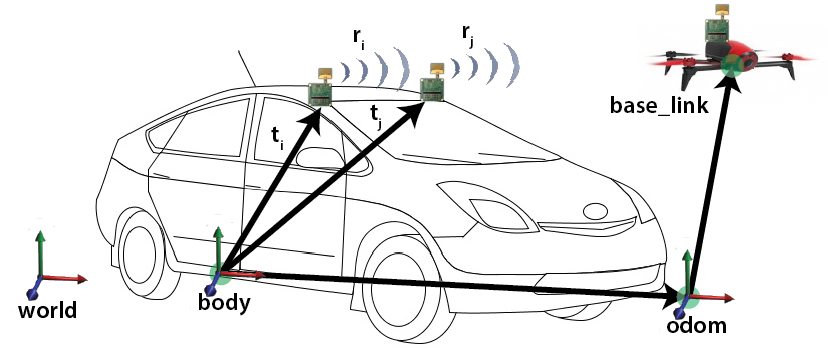
\includegraphics[width=0.7\textwidth]{foresight_frames}
  \caption{The frames and measurements of our system.}
  \label{fig:frames}
\end{figure}







